\section{Schema concettuale ristrutturato}
%Immagine: giorno su turno, codicepren mettere sotto
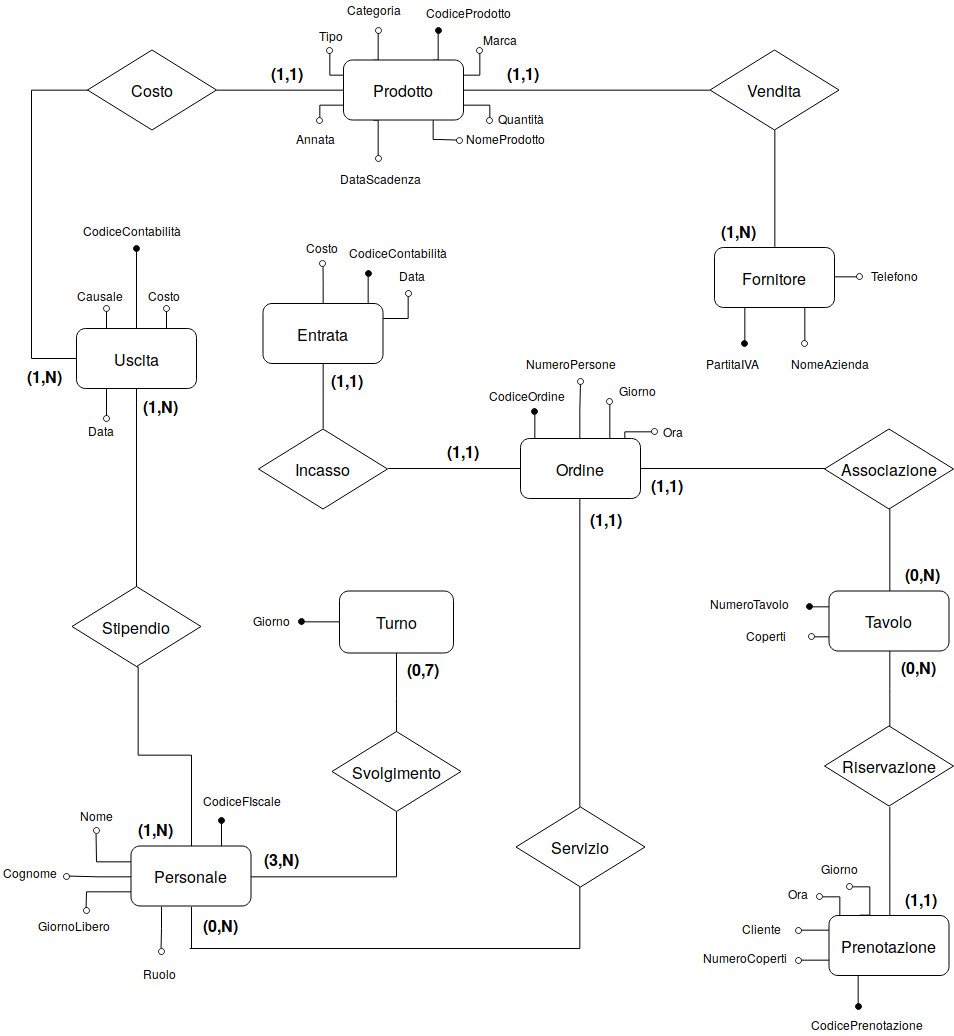
\includegraphics[width=1\textwidth]{doc/Ristrutturato}
\textbf{Eventuali note:}  
\begin{itemize}
    \item Dato che i sistemi tradizionali per la gestione per le basi di dati non consentono di rappresentare direttamente una \textit{generalizzazione} e tantomeno una gerarchia, risulta necessario trasformare questo costrutto in entita e relazioni. \\
    Per la nostra base di dati si e deciso di utilizzare tutti e tre i tipi di eliminazione:\\
    Accorpamento delle figlie della generalizzazione nel genitore, accorpamento del genitore della generalizzazione nelle figlie e sostituzione della generalizzazione con associazioni.\\ %manca un attributo nella prima generalizzazione
    Il primo metodo e stato utilizzato per l'eliminazione della gerarchia che coinvolge Vino, Superalcolico e Bevanda, per quella che coinvolge Cibo, Bevanda e Prodotto aggiungendo un attributo `Categoria` che distingue tra cibo e bevanda e anche per la generalizzazione che comprende Personale, Cuoco, Sommelier e Cameriere, dove in Personale e stato aggiunto un attributo `Ruolo`.\\
    Il secondo metodo e stato usato per accorpare Contabilita con le figlie Uscita ed Entrata.
    \item I sistemi di gestione di basi di dati richiedono generalmente di specificare una chiave primaria; nei casi in cui esistono entita per le quali sono specificati piu identificatori bisogna decidere quali di questi usare come chiave primaria. \\
    Dato che un identificatore composto da uno o pochi attributi e da preferire a identificatori costituiti da molti attributi e per gli stessi motivi, un identificatore interno e da preferire a uno esterno gli \textit{identificatori esterni} delle entita Ordine e Prenotazione vengono sostituiti con `CodiceOrdine` e `CodicePrenotazione`.
\end{itemize}

\section{Schema logico}
%Immagine
\subsection{Schema logico-relazionale} %Tabella(Attributi, .. )
\textbf{Fornitore}(\underline{PartitaIVA}, NomeAzienda, Telefono, ..), \\ \smallskip
\textbf{Prodotto}(\underline{CodiceProdotto}, Categoria, Marca, Tipo, Annata, DataScadenza, NomeProdotto, Quantita, ..), \\ \smallskip
\textbf{Uscita}(\underline{CodiceUscita},Costo, Data, Causale, ..), \\ \smallskip
\textbf{Entrata}(\underline{CodiceEntrata}, Costo, Data, ..), \\ \smallskip
\textbf{Personale}(\underline{CodiceFiscale}, Nome, Cognome, Ruolo, GiornoLibero, ..), \\ \smallskip
\textbf{Turno}(\underline{Giorno}, ..), \\ \smallskip
\textbf{Ordine}(\underline{CodiceOrdine}, NumeroPersone, Giorno, Ora, ..), \\ \smallskip %numero tavolo????????????
\textbf{Tavolo}(\underline{NumeroTavolo}, Coperti, ..), \\ \smallskip
\textbf{Prenotazione}(\underline{CodicePren}, NumeroCoperti, Cliente, Giorno, Ora, ..) %numero tavolo?

\section{Lista dei vincoli di integrità referenziale}
%Tabella con relazione e vincoli

